\documentclass{article}
\usepackage{amsmath}
\usepackage{tikz}
\usetikzlibrary{patterns}

\begin{document}

\begin{figure}[h]
    \centering
    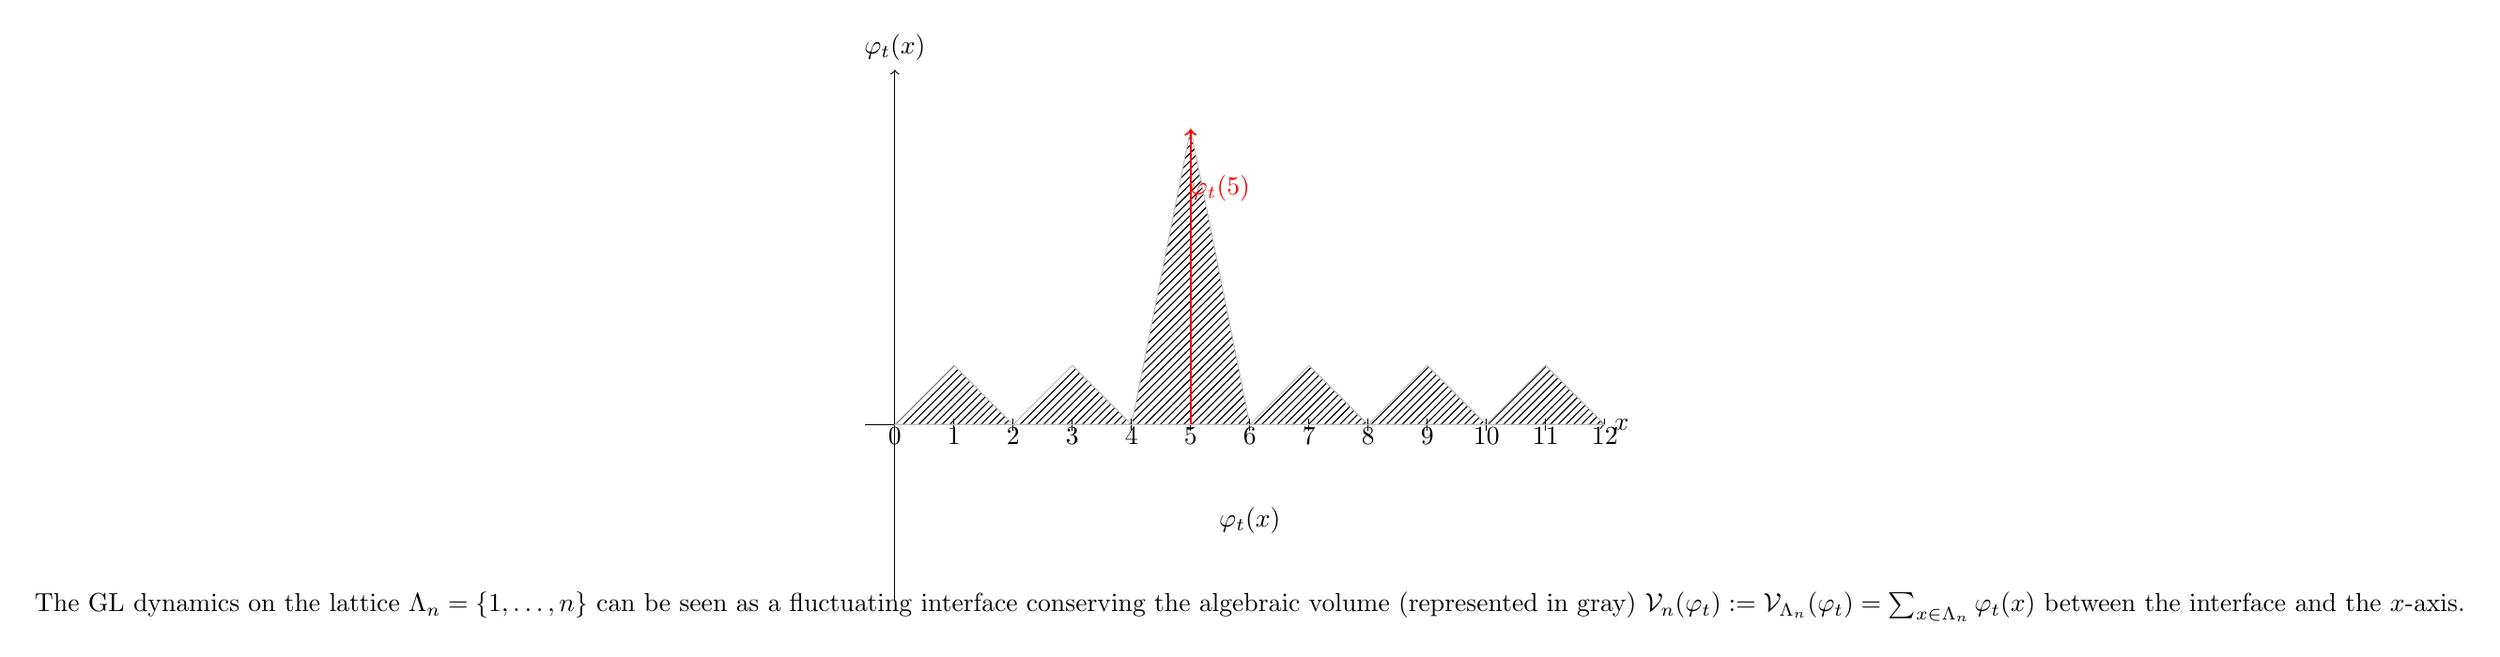
\begin{tikzpicture}[scale=0.8]
        % Axes
        \draw[->] (-0.5,0) -- (12,0) node[right] {$x$};
        \draw[->] (0,-3) -- (0,6) node[above] {$\varphi_t(x)$};
        
        % Grid lines
        \foreach \x in {0,...,11}
            \draw (\x,-0.1) -- ++(0,0.2);
        
        % Interface
        \filldraw[gray!50, pattern=north east lines] (0,0) -- (1,1) -- (2,0) -- (3,1) -- (4,0) -- (5,5) -- (6,0) -- (7,1) -- (8,0) -- (9,1) -- (10,0) -- (11,1) -- (12,0) -- cycle;
        
        % Interface points
        \foreach \x in {0,1,2,3,4,5,6,7,8,9,10,11,12}
            \draw (\x,0) -- ++(0,0.1) node[below] {\x};
        
        % Red arrow
        \draw[red, thick, ->] (5,0) -- (5,5);
        
        % Label for phi_t(5)
        \node at (5.5, 4) [red] {$\varphi_t(5)$};
        
        % Title
        \node at (6, -2) [above] {$\varphi_t(x)$};
        
        % Caption
        \node at (6, -3.5) [above] {
            The GL dynamics on the lattice $\Lambda_n = \{1, \ldots, n\}$ can be seen as a fluctuating interface conserving the algebraic volume (represented in gray) $\mathcal{V}_n(\varphi_t) := \mathcal{V}_{\Lambda_n}(\varphi_t) = \sum_{x \in \Lambda_n} \varphi_t(x)$ between the interface and the $x$-axis.
        };
    \end{tikzpicture}
    \caption{}
\end{figure}

\end{document}